
%(BEGIN_QUESTION)
% Copyright 2006, Tony R. Kuphaldt, released under the Creative Commons Attribution License (v 1.0)
% This means you may do almost anything with this work of mine, so long as you give me proper credit

The following differential pressure sensor uses a matched pair of strain gauges.  As the differential pressure increases, one strain gauge becomes compressed while the other becomes stretched.  A voltmeter registers the bridge circuit's imbalance and displays it as a pressure measurement.  The polarity symbols shown on the diagram next to the voltmeter show the polarity necessary to drive the meter upscale:

$$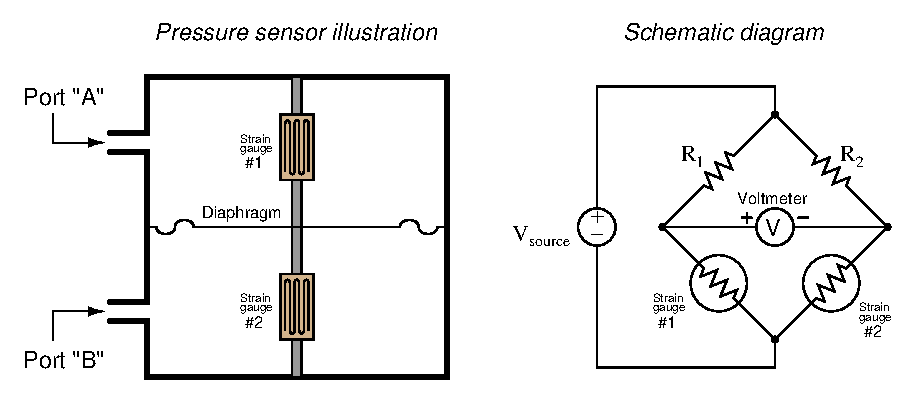
\includegraphics[width=15.5cm]{i00468x01.eps}$$

\begin{itemize}
\item{} Identify which port is the ``high'' pressure port
\item{} Identify what the voltmeter will register if fixed resistor $R_1$ fails open
\item{} Identify a component fault that would drive the voltmeter full upscale (``peg'' positive)
\item{} Identify another component fault that would drive the voltmeter full upscale (``peg'' positive)
\end{itemize}

\vfil 

\underbar{file i00468}
\eject
%(END_QUESTION)





%(BEGIN_ANSWER)

This is a graded question -- no answers or hints given!

%(END_ANSWER)





%(BEGIN_NOTES)

\begin{itemize}
\item{} Which port is the ``high'' pressure port: {\bf Port ``A''}
\item{} What will happen if fixed resistor $R_1$ fails open: {\bf Voltmeter will drive fully downscale (``peg'' negative)}
\item{} Identify a component fault that would drive the voltmeter full upscale (``peg'' positive):
\item\item{} {\bf (1) Strain gauge \#1 fails open} 
\item\item{} {\bf (2) Strain gauge \#2 fails shorted} 
\item\item{} {\bf (3) $R_1$ fails shorted}
\item\item{} {\bf (4) $R_2$ fails open}
\end{itemize}

\vskip 10pt

In order to determine which side is the ``high'' pressure port, we must first determine which strain gauge causes a positive signal changed when stretched.  From the bridge circuit schematic, we can see that strain gauge \#1 is the one which must increase resistance in order to generate a positive voltmeter reading.  Thus, port ``A'' must be the high pressure port, because this is the port where an applied pressure would place strain gauge \#1 under tension (and also compress strain gauge \#2, further causing a positive voltmeter indication).

\vskip 10pt

Any component failing in such a way as the make the left-hand terminal of the voltmeter more positive, or the right-hand terminal of the voltmeter more negative, will cause the voltmeter to register a greater positive voltage.

%(END_NOTES)


